\documentclass[12pt]{extarticle}
\usepackage{array}
\usepackage[T1]{fontenc}
\usepackage[Russian]{babel}
\usepackage{booktabs}
\usepackage{graphicx}
\usepackage{spreadtab}
\usepackage{numprint}
\usepackage[margin=3cm]{geometry}
\usepackage{float}
\usepackage{xfp}
\usepackage{amsmath} 
\usepackage{indentfirst}  
\begin{document}
\author{Осипов Александр Б06-604}
\title{Лабораторная работа 1.3.1. Определение модуля Юнга на основе исследования деформаций растяжения и изгиба}
\maketitle

\section{Цель}

Экспериментально получить зависимость между напряжением и деформацией (закон Гука) для одноосного растяжения и изгиба.
\vspace{5mm}

\section{Оборудование}

Первая часть: прибор Лермантова, проволки из исследуемого материала, зрительная труба со шкалой, набор грузов.

Вторая часть: стойка для изгибания балки, индикатор для измерения величины прогиба.

\vspace{5mm}

\section{Ход работы}

\subsection{Часть 1: Измерение коэффициента жесткости проволки}

Диаметр проволки:
d = 0.46 мм

Рычаг прибора:
r = 15 мм

Расстояние от шкалы до зеркальца:
h = 124 см

Длина проволки:
l = 177 см

\vspace{5mm}

\newpage
\textbf{\large{Эксперимент 1: измерение при увеличении нагрузки} }

\vspace{5mm}

\begin{spreadtab}{{tabular}{ccc}}
    @Номер замера & @Масса груза, г * 10 & @Смещение по шкале, см\\
    1& 5044& 19.6 \\
    2& 5044+2456& 22.3 \\
    3& 5044+2456+2453+2455& 27.3 \\
    4& 5044+2456+2453+2455+2461+2458 & 31.8 \\
    5& 5044+2456+2453+2455+2461+2458+2453+2456 & 36.2 \\
    6& 5044+2456+2453+2455+2461+2458+2453+2456+2455+2456 & 40.6 \\
    7& 5044+2456+2453+2455+2461+2458+2453+2456+2455+2456+2456 & 42.8 \\
\end{spreadtab}

\vspace{5mm}

\textbf{\large{Эксперимент 2 нагрузка уменьшается} }

\vspace{5mm}

\begin{spreadtab}{{tabular}{ccc}}
    @Номер замера & @Масса груза, г * 10 & @ Смещение по шкале, см \\
    1& 5044+2456+2453+2455+2461+2458+2453+2456+2455+2456+2456 & 42.8 \\
    2& 5044+2456+2453+2455+2461+2458+2453+2456+2455+2456 & 40.7 \\
    3& 5044+2456+2453+2455+2461+2458+2453+2456 & 36.3 \\
    4& 5044+2456+2453+2455+2461+2458 & 31.8 \\
    5& 5044+2456+2453+2455& 27.2 \\
    6& 5044+2456& 22.5 \\
    7& 5044& 19.5 \\
\end{spreadtab}

\vspace{5mm}

\textbf{\large{Результаты: }}

\begin{center}
  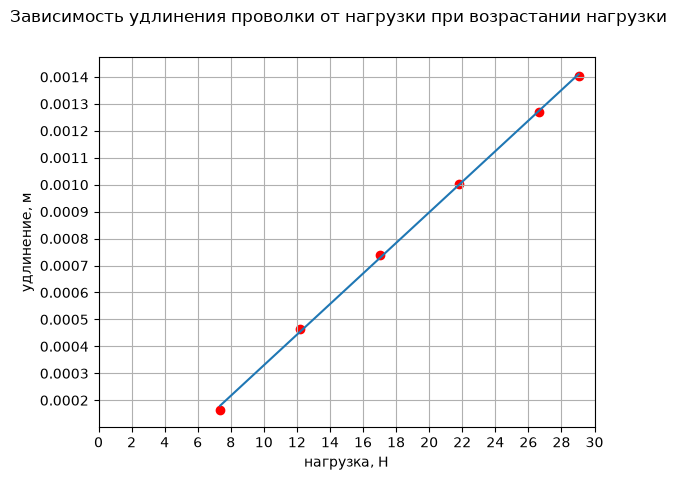
\includegraphics[scale=0.8]{../assets/1_3_1/lab_1_3_1_wire_increase.png}
\end{center}

\begin{center}
  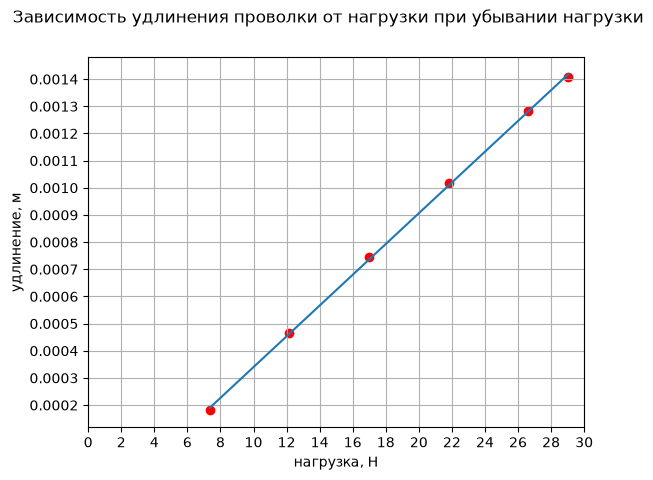
\includegraphics[scale=0.8]{../assets/1_3_1/lab_1_3_1_wire_decrease.png}
\end{center}

\vspace{5mm}
Коэффициент жёсткости 17639.891659067634 Н/м

Модуль Юнга 86.42143368814979 Гпа

\vspace{5mm}
Расчет ошибок измерения:

Используя формулу для $k$:
$$k = \frac{F \cdot 2h}{n \cdot r}$$

Рассчитаем по относительную ошибку для коэффициента жёсткости по формуле
относительной ошибки для функции нескольких переменных:
$$\sigma_k = \sqrt{\left(\frac{\partial k}{\partial h}\sigma_h\right)^2 + \left(\frac{\partial k}{\partial n}\sigma_n\right)^2 + \left(\frac{\partial k}{\partial r}\sigma_r\right)^2}$$

$\sigma_{h} = 0.001$

$\sigma_n = 0.001$

$\sigma_r = 0.001$

$$\varepsilon_k = \sqrt{\left(\frac{\sigma_h}{h}\right)^2 + \left(\frac{\sigma_n}{n}\right)^2 + \left(\frac{\sigma_r}{r}\right)^2}$$

\vspace{5mm}
Подставим значения:

$$\varepsilon_k = \sqrt{\left(\frac{0.001}{1.24}\right)^2 + \left(\frac{0.001}{2.7*10^{-2}}\right)^2 + \left(\frac{0.001}{0.015}\right)^2}$$

$$\varepsilon_k$$ = 0.067 (6.7\%)
\vspace{5mm}

\newpage

\subsection{Часть 2}

\vspace{5mm}

\textbf{\large{Определение модуля Юнга металлической балки}}

Расстояние между рёбрами призм:
l = 50,4 см

Материал балки:
металл

Ширина:
w = 21,4 мм

Толщина:
h = 4,4 мм

\vspace{5mm}
В ходе эксперимента балка в среднем имела остаточную деформацию 3-4 деления (0.03-0.04 мм)

\vspace{5mm}
Измерение 1 (нагрузка по центру):

\begin{spreadtab}{{tabular}{ccc}}
    @Номер замера & @Масса груза, г * 10& @Смещение стрелы прибора (количество делений)\\
    1& 5087& 67 \\
    2& 5000+5087 & 140 \\
    3& 5000+5087+5030 & 208 \\
    4& 5000+5087+5030+4679+5035 & 340 \\
    5& 5000+5087+5030+4679+5035+4618+4636 & 473 \\
\end{spreadtab}

\begin{center}
  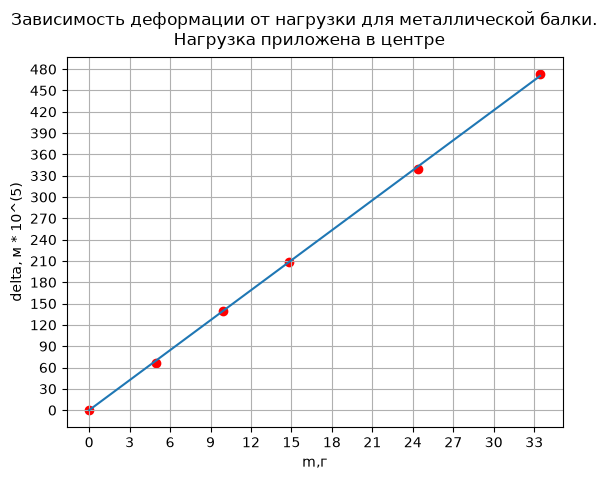
\includegraphics[scale=0.8]{../assets/1_3_1/balka_1.png}
\end{center}

E = 125 Гпа

\newpage
Измерение 2: смещение нагрузки на 2 см вправо:

\begin{spreadtab}{{tabular}{ccc}}
    @номер замера & @масса груза, г  делить на 10& @смещение стрелы прибора (деления)\\
    1& 5035& 69 \\
    2& 5035+4679& 130 \\
    3& 5035+4679+4618& 198 \\
    4& 5035+4679+4618+5087 & 261\\
    5& 5035+4679+4618+5087+4723+5020 & 403 \\
    6& 5035+4679+4618+5087+4723+5020+5030 & 466\\
\end{spreadtab}

\begin{center}
  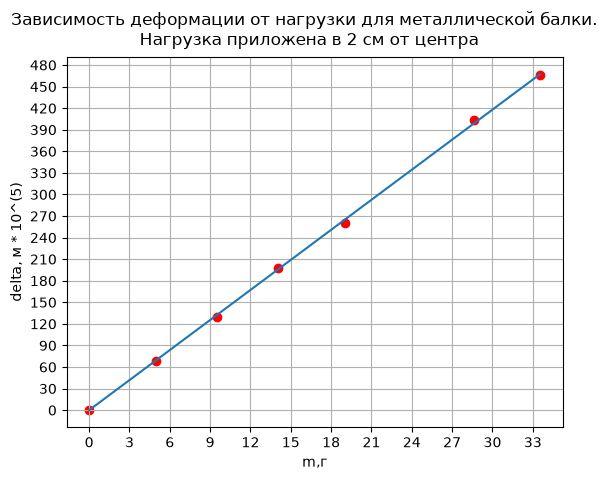
\includegraphics[scale=0.8]{../assets/1_3_1/balka_2.png}
\end{center}


\textbf{\large{Определение модуля Юнга деревяной балки 1}}

\vspace{5mm}
Измерение 3: 

Расстояние между рёбрами призм:
l = 50,4 см

Материал балки:
дерево

Ширина:
w = 20 мм

Толщина:
h = 10.1 мм

В ходе эксперимента балка в среднем имела остаточную деформацию 4-5 деления (0.04-0.05 мм).

E = 125 ГПа

\newpage
Измерение 3: нагрузка по центру

\begin{spreadtab}{{tabular}{ccc}}
    @номер замера & @масса груза, г делить на 10 & @смещение стрелы прибора (деления) \\
    1& 5035& 39 \\
    2& 5035+4679& 87 \\
    3& 5035+4679+4618& 138 \\
    4& 5035+4679+4618+5087 & 189 \\
    5& 5035+4679+4618+5087+4723+5020 & 284 \\
    6& 5035+4679+4618+5087+4723+5020+5030 & 339 \\
\end{spreadtab}

\begin{center}
  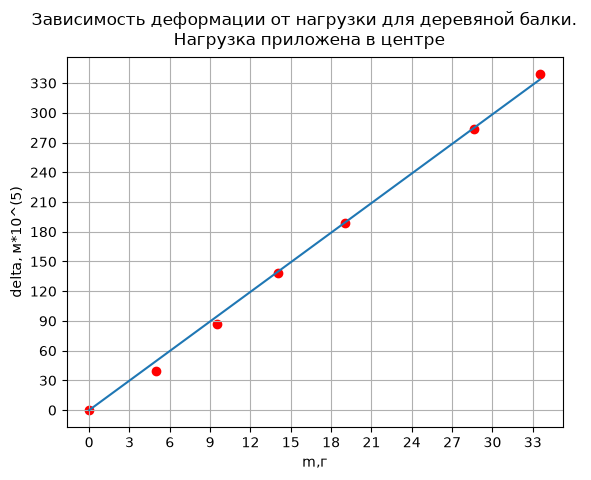
\includegraphics[scale=0.8]{../assets/1_3_1/balka_3.png}
\end{center}

E = 15.6 ГПа

\newpage
Измерение 4: смещение нагрузки на 4.8 см вправо:

\begin{spreadtab}{{tabular}{ccccccccccc}}
    @номер замера & @масса груза, г делить на 10 & @смещение стрелы прибора (деления) & @\text{mean}\\
    1& 5035& 34 & \\
    2& 5035+4679&  & \\
    3& 5035+4679+4618& 128 & \\
    4& 5035+4679+4618+5087 & 175 & \\
    5& 5035+4679+4618+5087+4723+5020 & & \\
    6& 5035+4679+4618+5087+4723+5020+5030 & 318 & \\
\end{spreadtab}

E = 15.4 ГПа

\begin{center}
  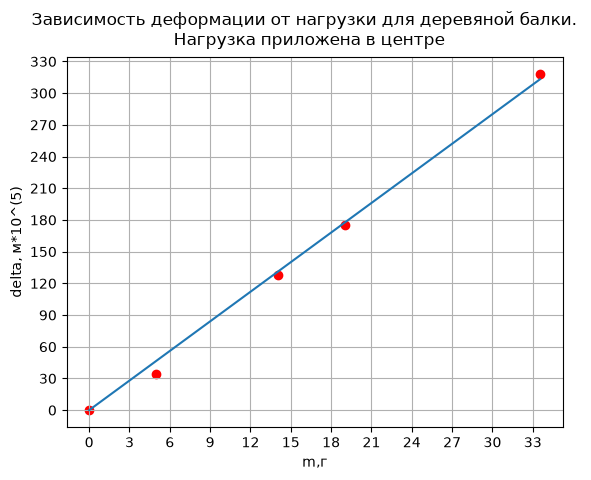
\includegraphics[scale=0.8]{../assets/1_3_1/balka_4.png}
\end{center}

\newpage
Измерение 5: нагрузка по центру, балка перевенута обратной стороной

\begin{spreadtab}{{tabular}{ccc}}
    @номер замера & @масса груза, г делить на 10 & @смещение стрелы прибора (деления)\\
    1& 5035& 49 \\
    2& 5035+4679& 98 \\
    3& 5035+4679+4618&  \\
    4& 5035+4679+4618+5087 & 176 \\
    5& 5035+4679+4618+5087+4723+5020 & \\
    6& 5035+4679+4618+5087+4723+5020+5030 & 322 \\
\end{spreadtab}

\begin{center}
  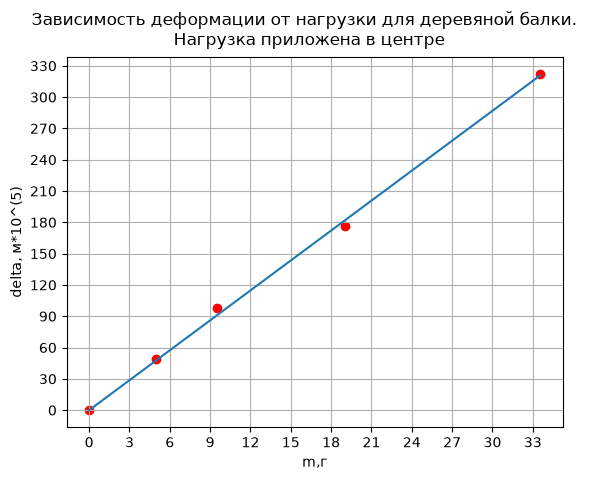
\includegraphics[scale=0.8]{../assets/1_3_1/balka_5.png}
\end{center}

E = 16.2 ГПа

\newpage
\textbf{\large{Определение модуля Юнга деревяной балки 2}}

Деревяная балка 2 
20 мм ширина
9,5 мм толщина

\begin{spreadtab}{{tabular}{ccccccccccc}}
    @номер замера & @масса груза, г делить на 10 & @смещение стрелы прибора (деления) & @\text{mean}\\
    1& 5035& 50\\
    2& 5035+4679&  109& \\
    3& 5035+4679+4618&  & \\
    4& 5035+4679+4618+5087 & 176 & \\
    5& 5035+4679+4618+5087+4723+5020 &  & \\
    6& 5035+4679+4618+5087+4723+5020+5030 & 331 & \\
\end{spreadtab}

\begin{center}
  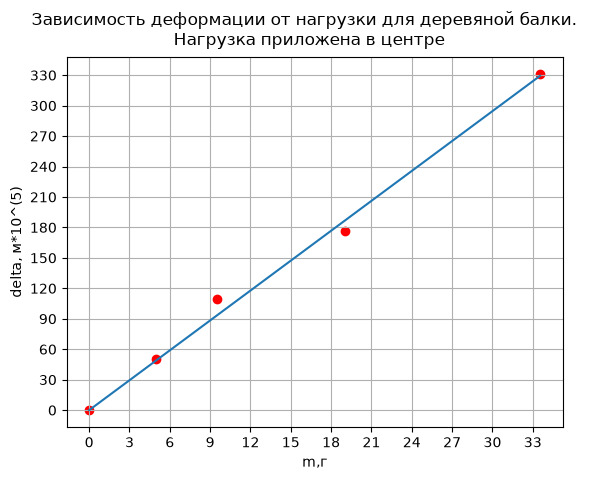
\includegraphics[scale=0.8]{../assets/1_3_1/balka_6.png}
\end{center}

E = 19 ГПа

\newpage
Эксперимент 1.3.2(2)

m(груза 1) = 377,5 г 

m(груза 2) = 373,1 г 

l = 1750+-2 мм 

d = 3,01 мм

Эксперимент 2 нагрузка уменьшается (читать снизу вверх)
\begin{spreadtab}{{tabular}{ccccccccccc}}
    @номер замера & @длина до груза, см & @амплитуда в ед на шкале &@количество периодов (время 10 колебаний/10)\\
    1 & 3 & 10 & 2,384 \\
    2 & 3 & 5 & 2,349 \\
    3 & 5 & 2,883 \\
    4 & 7 & 3,392 \\
    5 & 9 & 3,984 \\
\end{spreadtab}

Результаты:

\begin{center}
  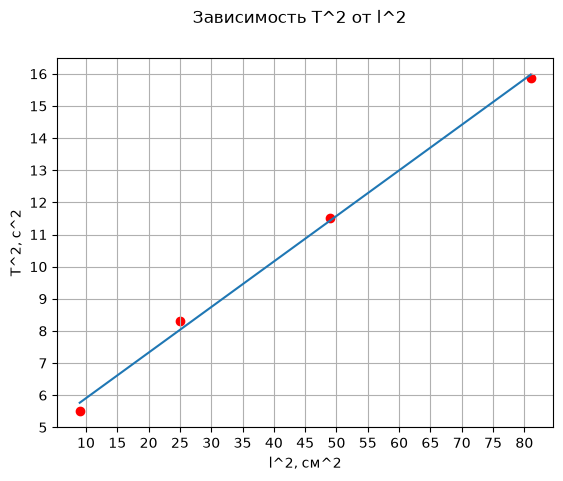
\includegraphics[scale=0.8]{../assets/1_3_1/rotation.png}
\end{center}

\end{document}
